% Desarrollo/Analisis de resultados

%% utilice capturas de pantalla para demostrar la funcionalidad, estas capturas de pantalla deben mostrar solo la información pertinente al paso correspondiente, en esta sección es muy importante realizar un análisis de la funcionalidad del programa (utilizar diagramas de flujo, diagramas de clase, etc) y un análisis de la funcionalidad electrónica (utilizando medidas del multímetro de voltajes y/o corrientes, osciloscopio y diagramas de onda). 

\subsection{Funcionalidad del programa}

La mayor parte del código empleado se basa en el tutorial \textit{Get Started With Machine Learning on Arduino} \cite{arduino}, con simples modificaciones para la integración de un tercer movimiento.  El tutorial enseña como entrenar y usar modelos de machine learning para el Arduino Nano 33 BLE Sense.  


    \subsubsection{Script de Arduino IMU\_Capture.ino}
    
        Este ejemplo utiliza la IMU (Unidad de Medición Inercial) integrada para comenzar a leer datos de aceleración y giroscopio y los imprime en el Monitor Serie durante un segundo cuando se detecta un movimiento significativo. También, el códgo permite utilizar el Visualizador Serie, herramienta del Arduino IDE, para graficar los datos. La biblioteca Arduino\_LSM9DS1 se usa para inicializar y leer los datos del IMU. Con la función de setup, se inicializa la comunicación serial con la consola así como con el IMU. También se verifica si la inicialización fue exitosa y se imprime el encabezado aX,aY,aZ,gX,gY,gZ para poder clasificar los datos.   \\

        Con el bucle loop, específicamente en el primer while, se está siempre esperando por la confirmación de aceleración en el movimiento de la placa. Al haber aceleración, se leen los 3 ejes respectivos y se estpa constantemente chequeando si la suma de las aceleraciones cruza el umbral de celeración. Cuando se cruza el umbral de aceleración, el conteo de muestras leídas se vuelve cero. \\

        El segundo while se cumple siempre y cuando la muestras de datos leídos sea menor al número de muestras. Es en este while donde se leen los datos del ejes respectivos del IMU para lo que es aceleración y los ejes respectivos del giroscopio. Todos estos datos son enviados por medio del puerto serial a la computadora, y son formateados para una fácil lectura. Por último, finalizada la lectura y toma de muestras, se agrega al puerto serial una línea vacía que significa que la toma de muestras ha finalizado y se puede realizar la siguiente. Este espacio vacío también es importante para el entrenamiento y uso del machine learning a aplicar más adelante.
        
    \subsubsection{Script de Python SensorDataCollector.py}
    
        Se crea un script de Python llamado SensorDataCollector.py para leer datos del puerto serial enviados por el código  Arduino IMU\_Capture.ino mencionado previamente. Luego, con este script de Python, se puede leer los datos desde el puerto serie, se procesa esta información extrayendo los valores numéricos de las lecturas realizadas del acelerómetro y el giroscopio, donde finalmente se guardan estos datos en un archivo CSV para realizar el análisis que sea necesario. En resumen, el sketch .ino funciona como un emisor de datos, y el script de Python actúa como el receptor de los valores generados.

    \subsection{Script de Python de Lab5\_Google\_Colab.ipynb} 
    Al script original \cite{arduino} se le agrega un \textit{gesture} más, que para este laboratorio es el movimiento de hacer un círculo con la mano.
    Este script de Python es específico para correr en Google Colab donde se entrena el modelo de aprendizaje automático utilizando los datos recopilados de la placa Arduino en el sketch IMU\_Capture.ino y del script SensorDataCollector.py. Los datos se encapsulan en documentos .csv entre 10-11 muestras por movimiento. 
    Colab proporciona un cuaderno Jupyter que permite ejecutar el entrenamiento de TensorFlow en un navegador web, y así evitar utilizar los recursos de nuestras portátiles. Luego, a partir del tutorial \cite{arduino}, se entrena el modelo a partir de machine learning siguiendo los siguientes pasos:

    \begin{enumerate}
        \item Configurar el entorno de Python: Se configuran las dependencias necesarias para el cuaderno. \cite{arduino}
        \item Cargar los datos de punch.csv, flex.csv y circulo.csv.
        \item Analizar y preparar los datos: Se analizan los archivos CSV y se transforman a un formato que se utilizará para entrenar la red neuronal. \cite{arduino}
        \item Construir y entrenar el modelo: Se construye y entrena un modelo de TensorFlow utilizando la API de alto nivel Keras. \cite{arduino} tf.keras es la API de alto nivel de TensorFlow para construir y entrenar modelos de aprendizaje profundo. Se utiliza para la creacion rapida de prototipos, la investigacion de vanguardia (estado-del-arte) y en producción. \cite{keras}
        \item Convertir el modelo entrenado a TensorFlow Lite: Se convierte el modelo al formato TFlite. \cite{arduino}
        \item Codificar el modelo en un archivo de encabezado de Arduino: El paso final del Colab genera el archivo model.h para descargar e incluir en nuestro proyecto de clasificación de gestos en el Arduino IDE. \cite{arduino}
    \end{enumerate}

    \subsection{Script de Arduino imu\_classifier.ino }

    Este script hace uso del IMU de 9 ejes presente en la placa para empezar a medir la orientación de la placa (datos del giroscopio) así como la aceleración. Cuando tiene los suficientes muestras de datos, hace uso del modelo TensorFlow Lite (Micro) o bien, del archivo \textit{modelo.h} para clasificar el movimiento ejecutado por el usuario y clasifica dicho movimiento entre los posibles: flexión, golpe o círculo. La correspondencia númerica según el movimiento ejecutado se refleja en terminal.
    Se tienen 3 simples movimientos registrados a identificar por el algoritmo: flexión, golpe y círculo; todos realizados con la mano del usuario. Una parte importante de este sketch es la biblioteca TensorFlow Lite Micro para Arduino, la cual está diseñada para ejecutar modelos de aprendizaje automático y la cual es compatible con la mayoría de las placas basadas en Arm Cortex M, como el Arduino Nano 33 BLE Sense. El repositorio se puede encontrar en \url{https://github.com/tensorflow/tflite-micro-arduino-examples#how-to-install}.

    


\subsection{Funcionalidad electrónica}

\subsubsection{Movimiento flex (inglés) o flexión}

En la figura \ref{flex1}, se tiene la posición inicial para el movimiento de flexión tipo levantando una mancuerna. Note la posición de la placa en la mano. Consecutivamente, el movimineto se hace rápido para  ``despertar'' el LSM9DS1 para que inice la toma de datos. La toma de datos se da en el puerto serial COM4 puesto que se utilizó Windows y estos datos pasan a escribirse en un archivo .csv a través del script de Python previamente mencionado. Un movimiento lento no hará que se inicie al toma de datos, sin embargo, esto se nota al monitorear la terminal tanto del Arduino IDE con la opción Serial Monitor, o bien, a través de arduino-cli (antes cerrar Arduino IDE) y monitorear el puerto desde esta terminal arduino-cli con el comando arduino-cli monitor -p COM4.

    \begin{figure}[H]
        \centering
        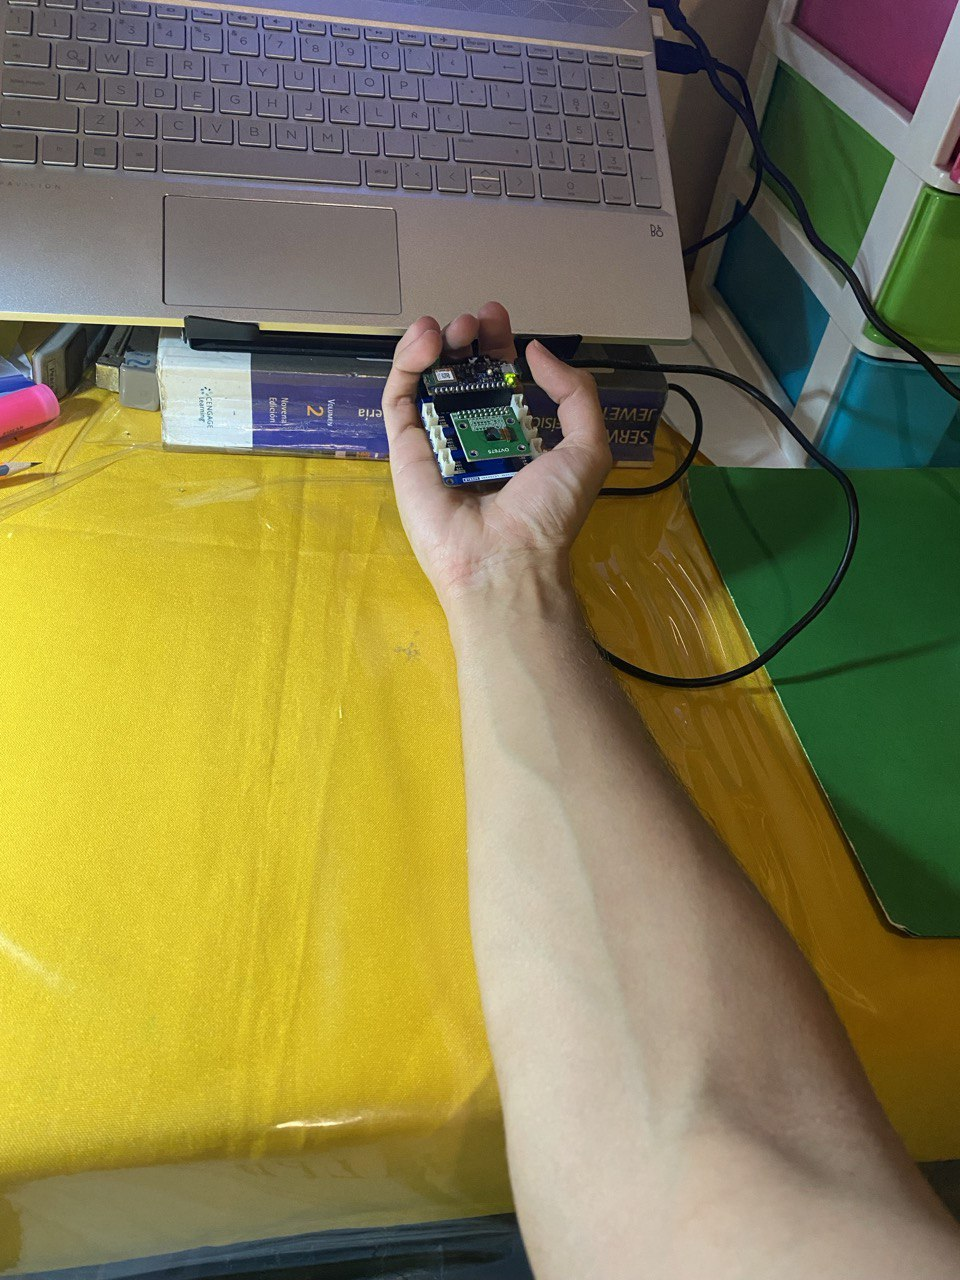
\includegraphics[width=0.5\linewidth]{pics/flex1.jpg}
        \caption{Posición inicial de la mano antes de hacer la flexión.}
        \label{flex1}
    \end{figure}
    
La figura \ref{flex3} presenta la posición final del movimiento. Este movimiento se realizó un total de 10 veces, lo cual fue suficiente debido a los altos porcentajes de eficiencia a la hora de identificar el movimiento presentes en los resultados en figura \ref{flex3}.

    \begin{figure}[H]
        \centering
        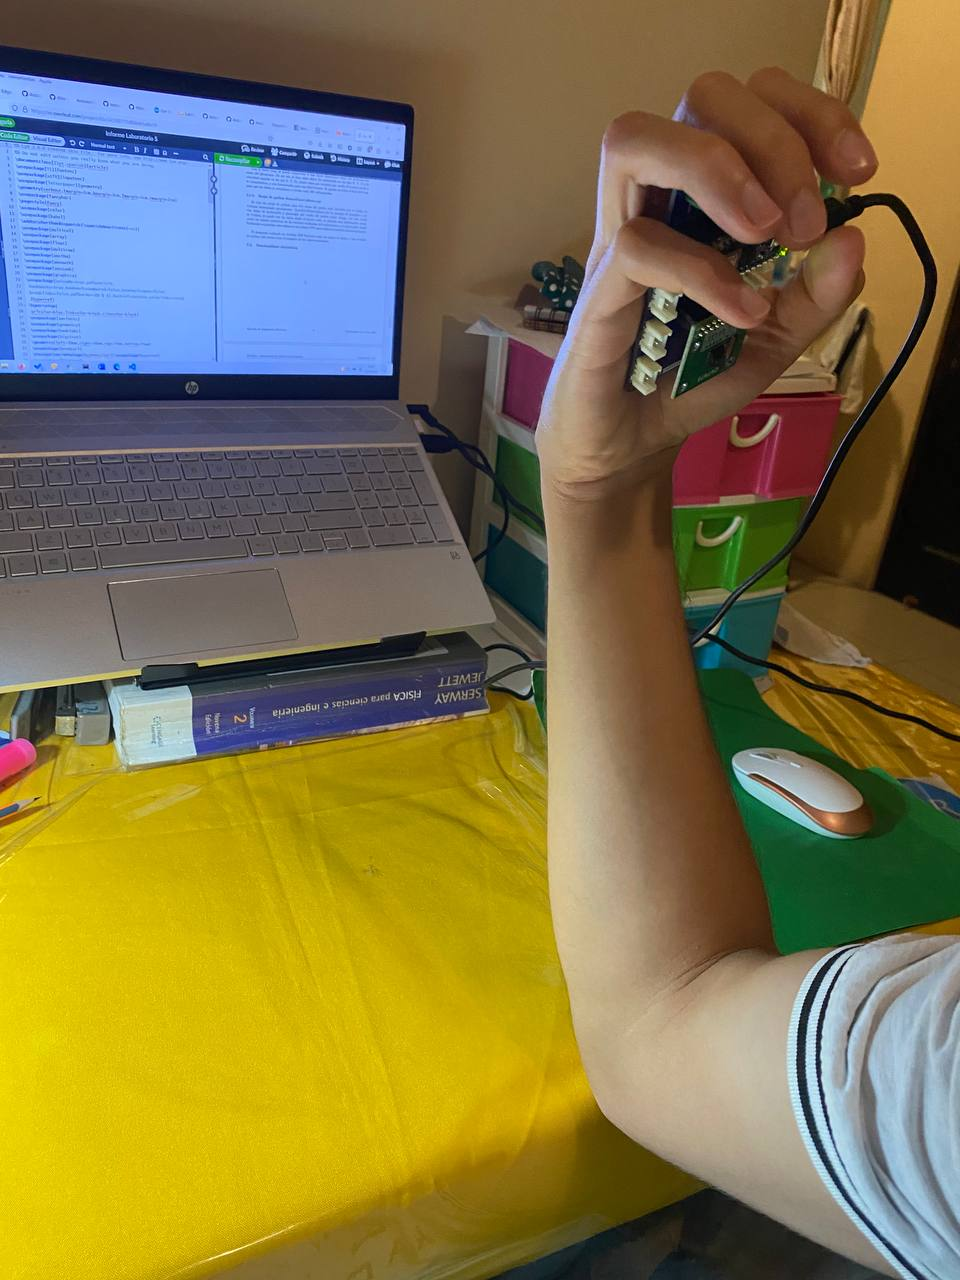
\includegraphics[width=0.5\linewidth]{pics/flex2.jpg}
        \caption{Posición final de la mano después de hacer la flexión.}
        \label{flex2}
    \end{figure}

En la figura \ref{flex3}, se encuentran los resultados en terminal luego de obtener el modelo.h a través del Google Colab discutido en sección 3.2. La figura \ref{flex3} muestra los resultados en ``porcentaje'' (un 0.999942 es igual a decir 99.9942\%) sumamente cercanos al 100\%, por lo cual, el modelo es exacto y preciso. En la figura se aprecian 3 resultados, en los cuales todos muestran un 99.99\% de identificación para el movimiento flexión.

    \begin{figure}[H]
        \centering
        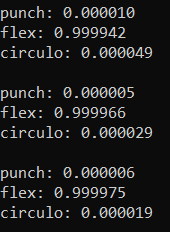
\includegraphics[width=0.3\linewidth]{pics/flex3.png}
        \caption{Resultados en terminal del movimiento flexión.}
        \label{flex3}
    \end{figure}
\subsubsection{Movimiento punch (inglés) o golpe}

A continuación, se analizará la toma de pruebas y analisis de resultados para el movimiento golpe. En la figura \ref{golpe1}, se observa la posición inicial del golpe, la mano derecha se ubica cerca del pecho del usuario. Note la posición del arduino. Luego, un súbito golpe hacia el frente sucede para activar la toma de datos y poderla observar terminal. 

\begin{figure}[H]
        \centering
        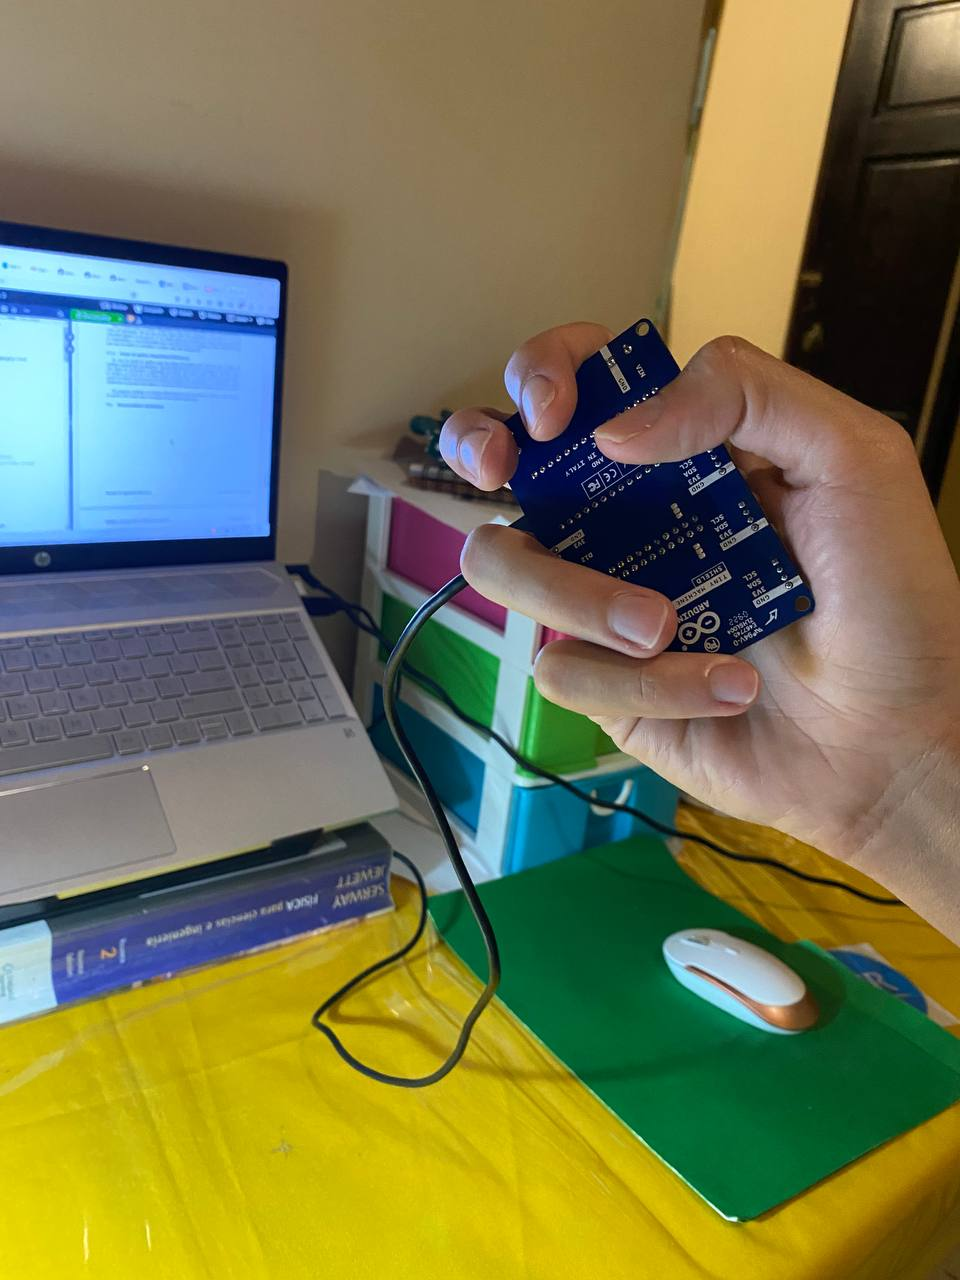
\includegraphics[width=0.5\linewidth]{pics/golpe1.jpg}
        \caption{Posición inicial de la mano antes de hacer el golpe.}
        \label{golpe1}
    \end{figure}

En la figura \ref{golpe2}, se observa la posición final del golpe hacia al frente, muy cerca de la laptop. La toma de muestras para este movimiento fue de 10-11 aproximadamente. Justo después de la posición final, hay que mover la mano hacia la posición final de forma lenta para no activar accidentalmente una nueva toma de datos.

    \begin{figure}[H]
        \centering
        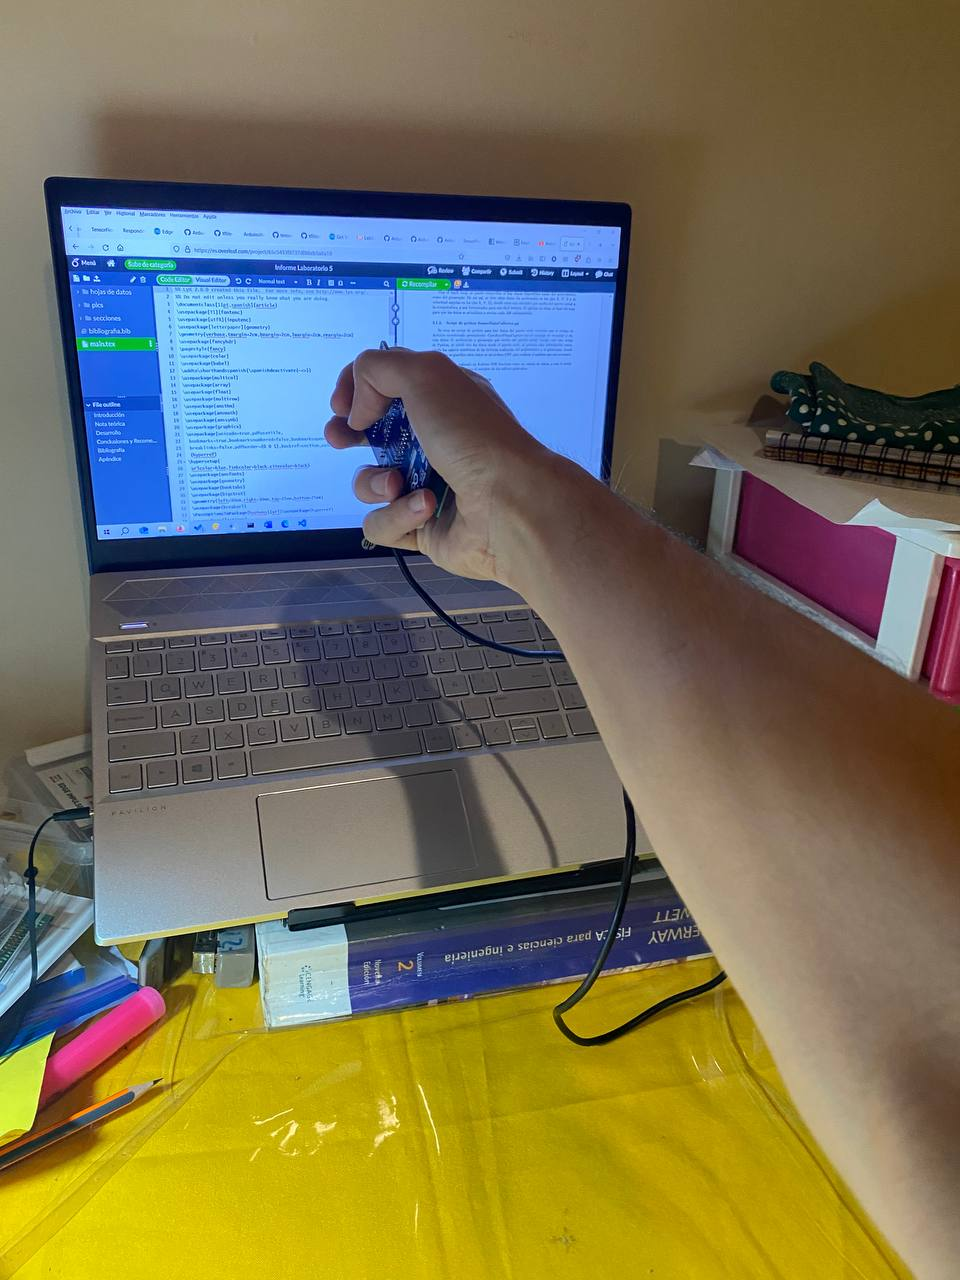
\includegraphics[width=0.5\linewidth]{pics/golpe2.jpg}
        \caption{Posición final de la mano después de hacer el golpe.}
        \label{golpe2}
    \end{figure}

En la figura \ref{golpe3}, se observan 4 resultados del movimiento golpe luego de subir el sketch con el modelo.h obtenido del Google Colab. Al igual que el analísis al movimiento de flexión, aquí se obtienen eficiencias al reconocimiento del movimiento mayores al 97\%. El modelo.h ha sido hasta el momento un modelo excelente capaz de reconocer el tipo de movimiento en prueba.

    \begin{figure}[H]
        \centering
        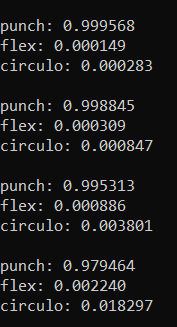
\includegraphics[width=0.3\linewidth]{pics/punch3.png}
        \caption{Resultados en terminal para el movimiento golpe.}
        \label{golpe3}
    \end{figure}

\subsubsection{Movimiento círculo}

El tercer y último movimiento puesto a prueba fue el movimiento de hacer un círculo con la mano derecha en el sentido antihorario, tal y como se aprecia en la figura \ref{circulo1}. En esta figura se muestra la posición inicial del arduino (ver forma en que se sujeta) y se muestra el recorrido a seguir a través de la flecha verde. El movimiento es súbito y rápido. Al igual que para los movimientos anteriores, se hizo un total de 10 pruebas para la creación del modelo con machine learning.

    \begin{figure}[H]
        \centering
        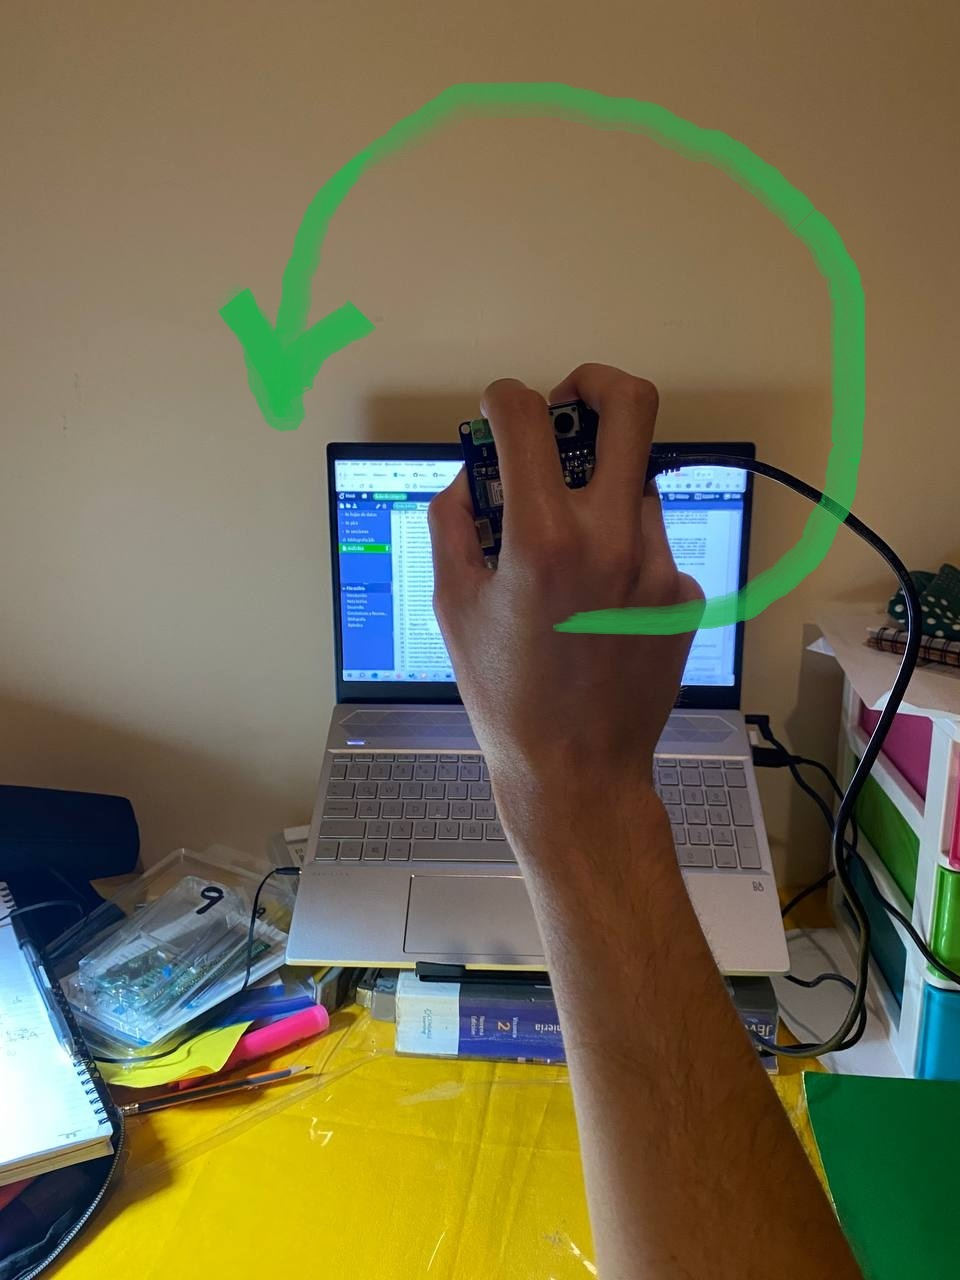
\includegraphics[width=0.5\linewidth]{pics/circulo.jpg}
        \caption{Movimiento del círculo en sentido antihorario.}
        \label{circulo1}
    \end{figure}

En la figura \ref{circulo2}, se presentan los resultados en terminal del movimiento círculo, o bien, el hacer un círculo con la mano. Se aprecian resultados de coincidencia del 99.82\%, al menos en los 3 resultados en figura \ref{circulo2}. Por lo tanto, el modelo.h entrenado a partir de las muestras y desarrollado a través del proceso de machine learning ha sido exitoso al reconocer los 3 movimientos discutidos en el presente laboratorio.

    \begin{figure}[H]
        \centering
        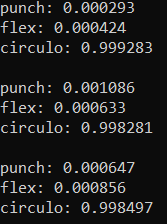
\includegraphics[width=0.3\linewidth]{pics/circulo2.png}
        \caption{Resultados en terminal para el movimiento círculo.}
        \label{circulo2}
    \end{figure}